% http://asi.insa-rouen.fr/fr/pages/le-stage-de-specialite?language=fr
% https://intranet.insa-rouen.fr/pilotage-et-organisation-de-letablissement/direction-generale/formations/rubriques/scolarite/guide-du-stage-ingenieur-1/guide-du-stage-ingenieur

\documentclass[12pt]{scrreprt}
%\pdfminorversion=4 % to avoid the error: "There was a problem reading this document (131)"

% Texte
\usepackage[utf8]{inputenc}
\usepackage[T1]{fontenc}
\usepackage[francais]{babel, varioref}
\usepackage[babel=true]{csquotes}
\usepackage{color}
\usepackage{minted}
\usepackage{caption}
\usepackage{subcaption}
\usepackage{afterpage}
\usepackage[super]{nth}
\usepackage{amssymb} % pour l'ensemble des réels
\usepackage[procnames]{listings}
\usepackage{color}
\usemintedstyle{trac}

\definecolor{keywords}{RGB}{255,0,90}
\definecolor{comments}{RGB}{0,0,113}
\definecolor{red}{RGB}{160,0,0}
\definecolor{green}{RGB}{0,150,0}
\lstset{
	language=Python,
	float=hbp,
	basicstyle=\ttfamily\small,
	identifierstyle=\color{colIdentifier},
	keywordstyle=\bf \color{colKeys},
	stringstyle=\color{colString},
	commentstyle=\color{colComments},
	columns=flexible,
	tabsize=3,
	frame=single,
	frame=shadowbox,
	rulesepcolor=\color[gray]{0.5},
	extendedchars=true,
	showspaces=false,
	showstringspaces=false,
	numbers=left,
	firstnumber=1,
	numberstyle=\tiny,
	breaklines=true,
	backgroundcolor=\color{hellgelb},
	captionpos=b
}

\definecolor{colFond}{rgb}{0.8,0.9,0.9}
\definecolor{hellgelb}{rgb}{1,1,0.8}
\definecolor{colKeys}{rgb}{0,0,1}
\definecolor{colIdentifier}{rgb}{0,0,0}
\definecolor{colComments}{rgb}{0,0.5,0}
\definecolor{colString}{rgb}{0.62,0.12,0.94}
\lstdefinestyle{myTextStyle} {
	language=TeX,
	float=hbp,
	basicstyle=\ttfamily\small,
	identifierstyle=\color{colIdentifier},
	keywordstyle=\bf \color{colKeys},
	stringstyle=\color{colString},
	commentstyle=\color{colComments},
	columns=flexible,
	tabsize=3,
	frame=single,
	frame=shadowbox,
	rulesepcolor=\color[gray]{0.5},
	extendedchars=true,
	showspaces=false,
	showstringspaces=false,
	numbers=left,
	firstnumber=1,
	numberstyle=\tiny,
	breaklines=true,
	backgroundcolor=\color{hellgelb},
	captionpos=b,
}

%%%%%%%%%%%%%%%%%%%%%
\usepackage{url}
\usepackage[top=2.1cm,bottom=2.2cm,left=2cm,right=2cm]{geometry}
\usepackage[final]{pdfpages}
%%%%%%%%%%%%%%%%%%%%%%%%%%%

%%%%%%%%%%% Pour sommaire cliquable %%%%%%%%%%
\usepackage{hyperref} % Créer des liens et des signets
\hypersetup{
	colorlinks=true, %colorise les liens
	breaklinks=true, %permet le retour à la ligne dans les liens trop longs
	urlcolor=blue, %couleur des hyperliens
	linkcolor=black, %couleur des liens internes
	citecolor=black,  %couleur des références
}
%%%%%%%%%%%%%%%%%%%%%%%%%%%%%%%%%%%%%%%%%%%%

% Images
\usepackage{float}
\usepackage{wrapfig}
\usepackage{graphicx}

% Tables
\usepackage{longtable}
\usepackage{booktabs}

% Couverture
\usepackage{templateINSA}
\initINSA

\renewcommand\infoBig{Monographie}
\renewcommand\infoSmall{DataTeam - 50W}
\title{Big Data and Tweet Streaming}
\author{Christophe \textsc{Cluizel} \and \textsc{Thibaud Dauce}}

\renewcommand\soustitre{Christophe \textsc{Cluizel} \& Thibaud \textsc{Dauce}}

\author{
	\textbf{} \\
	\textbf{}\\
	\textbf{} \\
	\textbf{Années:} 2014-2015 (ASI5)\\
	\textbf{Date:} \today\\
	\textbf{}\\
}

\newcommand\TODO[1]{\textcolor{red}{\textbf{#1}}}

%% -- Document
\begin{document}
	% titleINSA : Page de garde
	% #1 : descendre le titre du milieu (en mm)
	% #2 : lien de l'image de fond
	% #3 : décalage sur X de l'image de fond (en mm)
	% #4 : décalage sur Y de l'image de fond (en mm)
	% #5 : largeur de l'image de fond de #5 (en mm)
	% #6 : Crédit de l'image de fond
	\titleINSA{8}{images/AVARI-Next-Best-Content-Editor.png}{0}{110}{225}{Licence - AVARI.io}

	% sommaire
	\renewcommand{\contentsname}{Sommaire}
	\tableofcontents

	\chapter{Partie A}
		\section{A0}
  En tant qu'entreprise de statistiques, la compagnie Twitter Inc nous a demandé d'analyser les tweets d'internautes en temps réel afin de récupérer et d'illustrer le nombre de tweets par jour et par nationalité, ainsi que la taille des tweets en question. Cela leur permettra de mettre en place une infrastructure dynamique pour s'adapter à la charge selon l'heure de la journée. Ce projet a donc pour objectif d'améliorer un processus de développement en fournissant une solution d'analyse en temps réel.

\section{A1}
  \subsection{Mots-clés}
  \label{sub:Mots-clés}

    \begin{itemize}
      \item Tweet
      \item Spark streaming
      \item Parallélisation
      \item Visualisation
      \item Temps réel
      \item Profil utilisateur
      \item Data mining
      \item Big data
      \item Scalabilité
      \item Données
    \end{itemize}

  \subsection{Questions d'amorce}
  \label{sub:Questions d'amorce}

    \paragraph{Grappe de serveurs}
    \label{par:Grappe de serveurs}
    Une grappe de serveurs (ou \textit{cluster}) est un regroupement de machines permettant de dépasser les capacités d'une machine. Il existe quatre cas d'utilisation pour une grappe de serveurs.
    \begin{description}
      \item[Mise à niveau de l'infrastructure] Ce système permet d'ajouter rapidement de nouveaux serveurs peu puissants et donc peu chers afin d'améliorer les performances. Avec l'utilisation d'une unique machine, l'amélioration peut devenir très coûteuse dans le cas de très grosses configurations.
      \item[Disponibilité de l'infrastructure] La multiplication des machines permet de disposer d'une infrastructure très stable. En effet, dans le meilleur des cas, il n'existe pas de machine maîtresse dans la grappe, il n'y a donc pas de \textit{single point of failure}.
      \item[Répartition de la charge] Il est possible avec une grappe de serveurs de diriger les requêtes de traitement vers le serveur le moins encombré. Si les machines sont situées dans des pays différents, il est également possible d'améliorer les performances (en particulier la latence) en dirigeant l'utilisateur vers la machine la plus proche.
      \item[Mutualisation des ressources] L'un des avantages les plus recherché dans l'utilisation d'une grappe de serveurs est la mutualisation des ressources. Il est en effet possible de créer des machines virtuelles profitant de toutes les ressources de la grappe. Il est nécessaire tout de même de faire attention au réseau entre les serveurs qui peut très vite devenir un goulot d'étranglement.
    \end{description}

    \paragraph{L'écosystème Hadoop}
    \label{par:L'écosystème Hadoop}
    Apache Hadoop est aujourd'hui le framework de calcul distribué le plus connu. En effet, tout un écosystème de traitement de données s'est développé autour.
    \begin{description}
      \item[HDFS] HDFS est le principal composant d'Hadoop, c'est celui qui permet de stocker les données de façon distribuées.
      \item[HBase] HBase est une base de données distribuée sur HDFS qui s'interface parfaitement avec Hadoop.
      \item[Hive] Hive est également un outil très utilisé qui permet d'effectuer des requêtes de type SQL sur des données distribuées.
      \item[Pig] Pig est un outil proche de Hive qui permet d'interroger des données dans un langage spécifique (le Pig Latin).
      \item[Drill] Drill permet d'interroger des données distribuées (HDFS, S3…) et des bases de données NoSQL via des requêtes de type SQL. Il est utile pour sa diversité.
      \item[Impala] Impala permet également de faire des requêtes de type SQL sur des données distribuées. Il est plus rapide que Hive.
      \item[Flume] Flume est un gestionnaire de queue distribués. Il permet de déplacer et d'aggréger de grandes quantités de données en temps réel.
      \item[Mahout] Mahout met à disposition des algorithmes distribués de \textit{machine learning}.
      \item[Giraph] Giraph est un outil d'analyse de graphes (notamment utilisé par Facebook pour l'analyse du réseau social).
      \item[Mesos] Mesos permet d'abstraire les ressources des machines (virtuelles ou physiques). Il fournit une API pour que les outils de l'écosystème Hadoop puissent accéder à ces ressources.
      \item[ZooKeeper] Enfin, ZooKeeper est un outil de gestion de configurations. L'écosystème d'Hadoop étant très diversifié, il est intéressant d'avoir un outil permettant de faire le lien entre tous les autres outils.
    \end{description}
    Il existe de nombreux outils dans l'écosystème Hadoop et cette liste n'est pas exhaustive. De nombreux problèmes sont résolus par plusieurs d'entre eux car les solutions présentées sont souvent encore au stade de la recherche. Il est nécessaire de choisir le bon outil tout en sachant que des solutions plus performantes peuvent arriver très rapidement.

    Malgré la forte dominance d'Hadoop, le framework de calcul distribué Apache Spark est aujourd'hui plus rapide et profite d'une plus forte communauté. Apache Spark est également basé sur l'écosystème Hadoop et permet donc de profiter de tous les outils déjà développés. Certains modules natifs de Spark remplacent d'anciens outils comme pour Hive / Spark SQL ou Giraph / Spark GraphX.


\section{A2}
  \begin{description}
    \item[\href{http://spark.apache.org/streaming/}{Spark streaming}] Le site web d'Apache Spark contient de nombreuses informations et exemples concernant les algorithmes de Map / Reduce et de calcul distribués.
    \item[\href{https://dev.twitter.com}{Twitter Dev}] La documentation Twitter à destination des développeurs contient toutes les informations nécessaires à la récupération des tweets en temps réel (et en particulier la page \href{https://dev.twitter.com/streaming/overview}{sur l'API de Streaming})
    \item[\href{http://wiki.apache.org/hadoop}{Hadoop Wiki}] Le wiki d'Hadoop est également riche en informations sur les algorithmes de Map / Reduce. Il permet également d'accéder à de nombreux autres documentations concernant des projets liés potentiellement utiles tels que \href{https://cwiki.apache.org/confluence/display/Hive/Home}{Hive} ou \href{https://cwiki.apache.org/confluence/display/PIG/Index}{Pig}.
  \end{description}

\section{A3}
  \begin{itemize}
    \item \href{http://www.amazon.fr/Real-Time-Analytics-Techniques-Visualize-Streaming/dp/1118837916/ref=sr_1_7?s=english-books&ie=UTF8&qid=1446301986&sr=1-7&keywords=streaming}{Real-Time Analytics: Techniques to Analyze and Visualize Streaming Data}. Chapitre 1: ``Introduction to Streaming data''
    \item \href{http://www.amazon.com/Learning-Spark-Lightning-Fast-Data-Analysis/dp/1449358624/ref=sr_1_1?ie=UTF8&qid=1446301706&sr=8-1&keywords=apache+spark}{Learning Spark: Lightning-Fast Big Data Analysis}. Chapitre 10: ``Spark Streaming''
    \item \href{http://www.amazon.fr/Learning-Real-time-Processing-Spark-Streaming-ebook/dp/B015Q7I3NM/ref=sr_1_2?s=english-books&ie=UTF8&qid=1446301986&sr=1-2&keywords=streaming}{Learning Real-time Processing with Spark Streaming}. Chapitre 2: ``Architecture and Components of Spark and Spark Streaming''
  \end{itemize}

\section{A4}
  \subsection{Apache}

    La fondation Apache est une organisation à but non lucratif dont l'objectif est de développer des logiciels open-source. Le logiciel le plus connu est sans aucun doute le serveur web Apache. Tout projet open-source sous licence Apache 2 peut devenir un projet de la fondation Apache après une période d'incubation. \\

    De nombreux logiciels de traitement de données sont soutenus par la fondation dont Apache Hadoop, Apache Spark, Apache Lucene ou encore Apache Kafka. Les frameworks de calcul Hadoop et Spark sont aujourd'hui les plus utilisés dans le monde de l'analyse de masse de données. Apache Lucene est le moteur d'indexation utilisé par tous les grands projets open-source comme par exemple les moteurs de recherche Apache Solr et ElasticSearch. Apache Kafka est un système de queue de messages utilisé par plusieurs grandes entreprises comme Linkedin, Netflix ou Spotify.

  \subsection{Google}

    Google est actuellement le plus grand moteur de recherche du monde. Son business model est basé sur la publicité et les données utilisateurs. Cette particularité explique que Google soit la première entreprise à avoir rencontré des problèmes liés aux masses de données. La première contribution de Google a été faite sur l'analyse de masses de données de manière distribuée avec le paradigme de MapReduce. Ce type de programmation est expliqué dans un article de recherche de 2004 \href{https://www.usenix.org/legacy/publications/library/proceedings/osdi04/tech/full_papers/dean/dean_html/index.html}{MapReduce: Simplified Data Processing on Large Clusters}.\\

    Deux ans plus tard, Google va contribuer à nouveau sur les problématiques de masses de données en dévoilant BigTable, un système de stockage de données distribué à nouveau dans un article de recherche \href{http://static.googleusercontent.com/external_content/untrusted_dlcp/research.google.com/en/us/archive/bigtable-osdi06.pdf}{Bigtable: A Distributed Storage System for Structured Data}. Ces deux articles vont être la base des frameworks d'analyse de données Hadoop et Spark qui exploite le paradigme MapReduce. Les données sont stockées au format HDFS, un format dérivé de la solution BigTable propriétaire de Google.

  \subsection{Amazon}
    Amazon.com est une société de commerce électronique. En 2002, elle lance un nouveau produit appelé Amazon Web Services (AWS) permettant d’accéder à des fonctions latentes sur son site web. Ce nouveau produit va être un regroupement de services très utiles pour les entreprises intéressées dans le domaine de la masse de données. Tout d'abord avec Amazon Simple Storage Service (Amazon S3), un service de stockage de fichier volumineux. Il est possible de stocker très facilement des teraoctects de données dans S3 et de les analyser avec Hadoop ou Spark. Puis avec un système de serveurs virtualisé à la demande: Amazon Elastic Compute Cloud (Amazon EC2). \\

    Ce service permet de déployer des applications très facilement et de faire évoluer la puissance de calcul nécessaire en fonction du besoin en quelques clics. En 2013, Amazon dévoile Redshift, une base de données de type SQL permettant de traiter des masses de données efficacement. AWS permet aussi avec Amazon Elastic MapReduce (Amazon EMR) de traiter ses données via un cluster Hadoop ou Spark. Les prix très attractifs d'AWS peuvent expliquer l'engouement actuel pour ces technologies car de nombreuses entreprises ont pu se lancer dans des analyses sans investir des sommes astronomiques dans les machines et la configuration des clusters.

  \subsection{Smile}
    \href{http://www.smile.fr/}{Smile} est le leader français de l'intégration de logiciels open-source. Il propose des livres blancs disponibles gratuitement dans de nombreux domaines. Pour notre projet, nous avons choisi le livre blanc \href{http://www.smile.fr/Livres-blancs}{``Search Engines and E-merchandising: The State of the Art''} afin d'illustrer les possibilités des moteurs de recherche. Cet état de l'art ne correspond pas exactement à notre domaine d'application, mais expose plusieurs alternatives que nous aurions pu utiliser pour traiter nos tweet.

\section{A5}
  \begin{enumerate}
    \item Time behaviour
    \item Resource utilization
    \item Installability
  \end{enumerate}

\section{A6}
  \begin{enumerate}
    \item Time behaviour
      \begin{itemize}
        \item Response time (Internal)
        \item Task time
        \item Response time for display on Kibana - unit: second.
      \end{itemize} \bigskip

      Les \emph{response time} et \emph{task time} seront mesurés à l'aide d'un ``tic-toc'', c'est-à-dire la différence entre le timestamp avant et après l'exécution d'une fonction, d'un groupe de fonctions ou d'une tâche. \\

    \item Resource utilization
      \begin{itemize}
        \item Transmission capacity
        \item Number of memory related errors
        \item CPU usage - unit: percentage from total.
      \end{itemize} \bigskip

    \item Installability
      \begin{itemize}
        \item Number of installation steps
        \item Number of set-up operations
        \item Number of architectures which can be used as workers for Spark computation - unit: number
      \end{itemize} \bigskip
  \end{enumerate}

\section{A7}


  \chapter{Partie B}
    \section{B1}
\label{sec:B1}

Plusieurs approches techniques existent dans le domaine du streaming de données. Nous allons travailler avec des tweets mais il est possible d'appliquer toutes ces techniques dans d'autres domaines.\\

\subsection{Envoi des données pour analyse}
\label{sub:Envoi des données pour analyse}

  Tout d'abord, la première solution technique existante est l'envoi des données au fur et à mesure de leur arrivée. Dans notre cas: Twitter envoie chaque tweets au fur et à mesure de leur émission sur ce que l'on appelle un \textit{endpoint}. L'envoi de chaque tweet peut-être effectué suivant plusieurs protocoles différents comme HTTP pour le plus connu ou encore par un protocole créé spécialement pour l'application via de simples sockets réseaux.\\

  \paragraph{Avantage de la solution}
  \label{par:Avantage de la solution}
  Le principal avantage de cette technique est la rapidité du transfert de l'information. Les tweets sont traité à la même vitesse que leur création et l'information créé est donc réellement en temps réel (sans compter les temps de transfert de l'information de Twitter à notre programme de traitement ni le temps de traitement).

  \paragraph{Inconvénients de la solution}
  \label{par:Inconvénients de la solution}
  Cet avantage peut se transformer en inconvénient si l'\textit{endpoint} n'est pas capable d'absorber l'information assez rapidement. Au vu de la quantité de tweets envoyés sur Twitter, il est très compliqué de concevoir un système capable de réagir à la masse de données reçues. Dans le cas où le système ne permet plus de traiter les tweets, il cesse de répondre et les tweets envoyés par Twitter sont donc perdus.\\

  \paragraph{Outils pratiques}
  \label{par:Outils pratiques}
  Twitter ne propose pas actuellement de sytème d'\textit{endpoint}. Ce choix est facilement compréhensible au vu des inconvénients évoqués dans le paragraphe précédent. Il est par contre possible de mettre en place ce genre d'architecture pour des volumes de données moindres comme par exemple lors de l'exécution de l'envoi d'un message sur \href{https://slack.com/}{Slack} ou IRC (plateformes de messagerie instantanée). L'\textit{endpoint} peut dans ce cas exécuter des programmes spécifiques en fonction du message reçu.

\subsection{Utilisation de queues de messages}
\label{sub:Utilisation de queues de messages}

  Afin de résoudre le problème de la masse de tweets reçue par l'\textit{endpoint}, il est possible d'utiliser des queues de messages. Ces queues de messages n'ont pas vocations à traiter les données mais seulement les stocker en attendant la consommation.\\

  Avec cette solution technique, l'action de traitement ne reçoit plus les tweets en temps réel mais peut venir les récupérer dès qu'elle en a besoin dans la queue de messages. Nous ne sommes plus dans une situation de réception mais bien de récupération de l'information.\\

  \paragraph{Avantages de la solution}
  \label{par:Avantages de la solution}
  Cette solution permet de mieux réguler le flux de tweets car la queue n'a plus de problèmes pour absorber la masse de tweets envoyés car elle ne traite pas l'information. Le programme de traitement quant-à-lui peut récupérer l'information dès qu'il en a besoin. Le traitement est donc mieux réparti entre les périodes avec un fort volume de tweets (ou le traitement va prendre du retard) et les périodes de faible volume de tweets (ou le traitement va prendre de l'avance).

  \paragraph{Inconvénients de la solution}
  \label{par:Inconvénients de la solution}
  L'utilisation de la queue est tout de même limitée en terme d'espace de stockage. En effet, si le retard accumulé par le traitement devient trop important et qu'il devient impossible de stocker les tweets dans la queue (par manque de RAM pour une queue en mémoire vive ou d'espace disque pour une queue persistée sur disque), il est nécessaire de supprimer des anciens tweets ou de refuser des nouveaux tweets. Une information est donc perdue.

  \paragraph{Outils pratiques}
  \label{par:Outils pratiques}
  De nombreux outils de queues de messages existent. Il est possible d'utiliser Apache Flume ou Apache Kafka en auto-hébergé. Il est également possible de profiter de l'offre cloud d'AWS nommé Amazon Kinesis. Ces trois outils fonctionnent de la même manière: une source de données (Twitter dans notre cas), un tuyau stockant les tweets et un puit (notre programme de traitement).\\

  Ces trois outils sont des queues de messages distribuées. Cela signifie que ces programmes peuvent fonctionner sur plusieurs machines physiques ou virtuelles. Concernant Amazon Kinesis, l'architecture fonctionne par \textit{shards} qui sont des tuyaux distribués. Il faut donc gérer plusieurs consommateurs de la queue différents. Ces consommateurs ne vont pas accéder à toute l'information mais seulement une partie des tweets. Dans notre cas, les tweets sont des événements totalement indépendants cette multitude de consommateurs est donc sans importance. Dans le cas où les événements mis en queue pourrait être liés entre eux, deux solutions sont possibles: agréger les messages avant l'insertion dans la queue ou choisir une clé de partitionnement permettant d'insérer les messages liés dans le même tuyau et ainsi les traiter avec le même consommateur.

\subsection{Traitement des données de manière distribuée}
\label{sub:Traitement des données de manière distribuée}

  Nos queues de messages sont distribuées pour permettre de meilleures performances et une facilité dans l'amélioration de la puissance de stockage de la queue. Il est très intéressant également de travailler sur un programme de traitement des données distribué. En effet, il serait donc possible d'améliorer les perforances et les temps de calcul de notre programme en ajoutant de nouvelles machines.\\

  Pour permettre l'utilisation de machines distribuées, il est nécessaire que les données ainsi que l'algorithme soient distribués. Le pattern le plus réputé dans le domaine est celui du Map / Reduce (figure \ref{mapreduce}). Dans ce pattern, deux opérations sont définies: les opérations de \textit{mapping} qui s'exécutent en local sur chaque machine et permettre d'exploiter toute la puissance du distribué, et les opérations de type \textit{reduce} qui permette d'aggréger les résultats de toutes les machines sur la machine principale afin de les sauvegarder ou les exploiter. Cette dernière opération n'étant pas distribué, il faut faire particulièrement attention aux volumes de données remontés par les opérations de type \textit{reduce} afin de prévenir tout problème au niveau de la machine principale.

  \begin{figure}
    \centering
    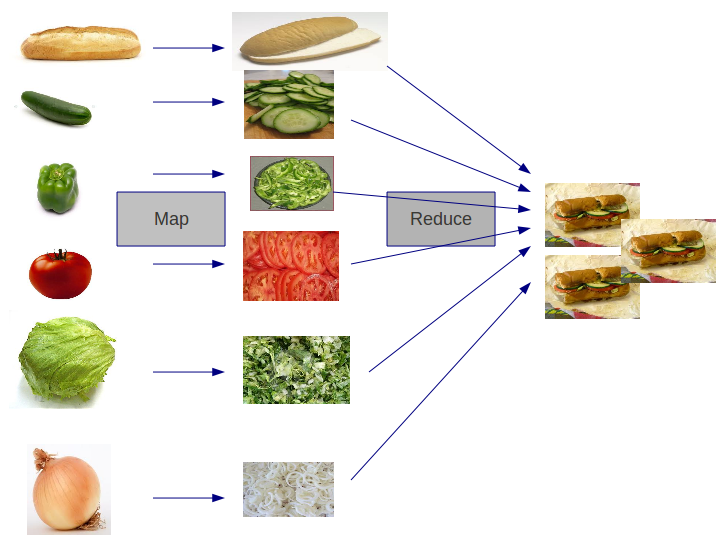
\includegraphics[width=0.8\textwidth]{images/mapreduce.png}
    \caption{Concept Map / Reduce expliqué à l'aide d'un sandwich.}
    \label{mapreduce}
  \end{figure}


\section{B2}
\label{sec:B2}
  \subsection{Spark Streaming}
  Afin de garantir un traitement distribué, il est possible d'utiliser le framework Apache Spark et plus précisément Spark Streaming pour traiter le flux de messages en temps réel ou de façon continue. Cet outil possède une bibliothèque (\emph{spark-streaming-twitter\_2.10}) permettant de communiquer directement avec l'API de Twitter. Il n'y a aucune restriction pour l'utilisation d'Apache Spark et sa bibliothèque, car ce sont des logiciels \emph{Open Source}.



  \subsection{??? En http à la main ?????}


\section{B3}
\label{sec:B3}
  \subsection{Spark Streaming}
    Afin de gérer le flux continu de données, Spark streaming va discrétiser le flux en \emph{batch}, c'est à dire en tranches d'informations. Ensuite, Spark va pouvoir effectuer les traitements ou calculs sur chacun de ces \emph{batch} de données de manière individuelle. La figure~\ref{streaming_flow} illustre ce découpage de flux de données. \\

  \begin{figure}
    \centering
    
\includegraphics[width=0.8\textwidth]{images/streaming-flow.png}
    \caption{Découpage du flux de données par Spark Streaming}
    \label{streaming_flow}
  \end{figure}

  Le flux n'est donc plus continue mais représenté par une couche d'abstraction appelée \emph{Discretized Stream} ou \emph{Dstream}. Chaque \emph{batch} peut être traité de manière indépendante et donc parallélisé. Par exemple, si l'on cherche à récupérer les mots d'un flux de lignes de texte, Spark va créer des \emph{batch} avec un certain nombre de lignes qui seront ensuite analysées individuellement pour obtenir les mots qui composent ces lignes de texte. La figure~\ref{streaming_dstream_get_word} présente cet exemple. Un grand nombre d'opérations peuvent être réalisés sur ces \emph{batch} de données, comme par exemple \emph{map}, \emph{reduce}, \emph{filter}, \emph{union}, \emph{count}… \\

  \begin{figure}
    \centering
    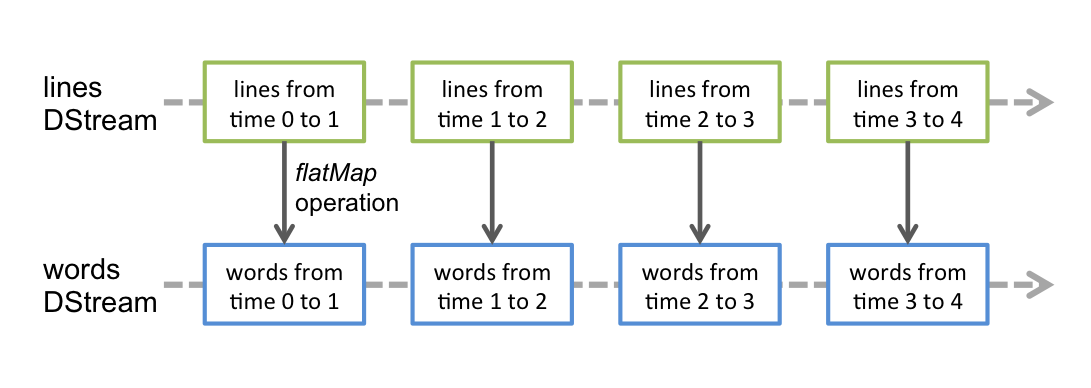
\includegraphics[width=0.8\textwidth]{images/streaming-dstream-ops.png}
    \caption{Exemple de récupération de mots par \emph{batch}}
    \label{streaming_dstream_get_word}
  \end{figure}

  Le flux étant discrétiser, Spark Streaming fournit des paramètres afin de régler la taille de la fenêtre de discrétisation, ainsi que l'intervalle entre deux lancements de calculs. Sur la figure~\ref{principe_de_fenetre_spark_streaming}, nous pouvons observer une taille de fenêtre d'une unité de temps entre chaque \emph{batch} (en vert), une taille de fenêtre de discrétisation regroupant les \emph{batch} de trois (en jaune) et un intervalle de deux entre chaque lancements de calculs sur les fenêtres de discrétisation (en rouge).

  \begin{figure}
    \centering
    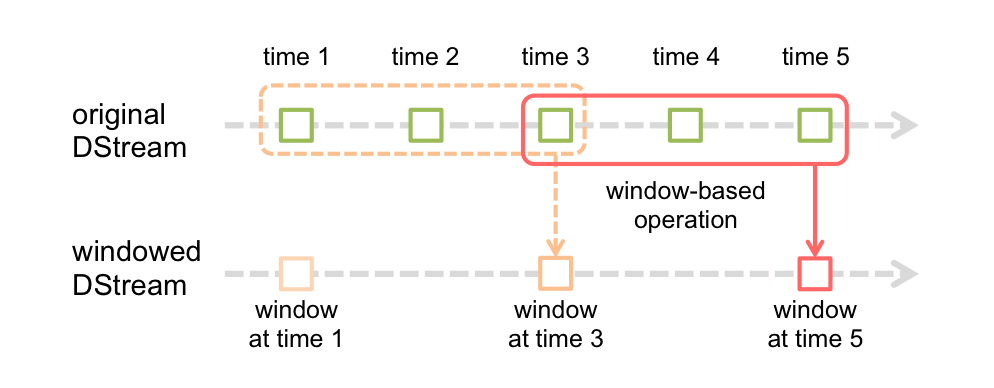
\includegraphics[width=0.8\textwidth]{images/streaming-dstream-window.png}
    \caption{Principe de fenêtrage}
    \label{principe_de_fenetre_spark_streaming}
  \end{figure}


\section{B4}
\label{sec:B4}
  Afin de comparer les deux solutions choisies, il convient de mettre en place un certain nombre de métriques de comparaison basées sur les indicateurs énoncés dans la partie~\ref{sec:A6}:

  \begin{itemize}
    \item ??????
    \item ??????
  \end{itemize}


\section{B5}
\label{sec:B5}
  La figure~\ref{WBS} représente notre \emph{Work Breakdown Structure} pour nos deux prototypes.

  \begin{figure}
    \centering
    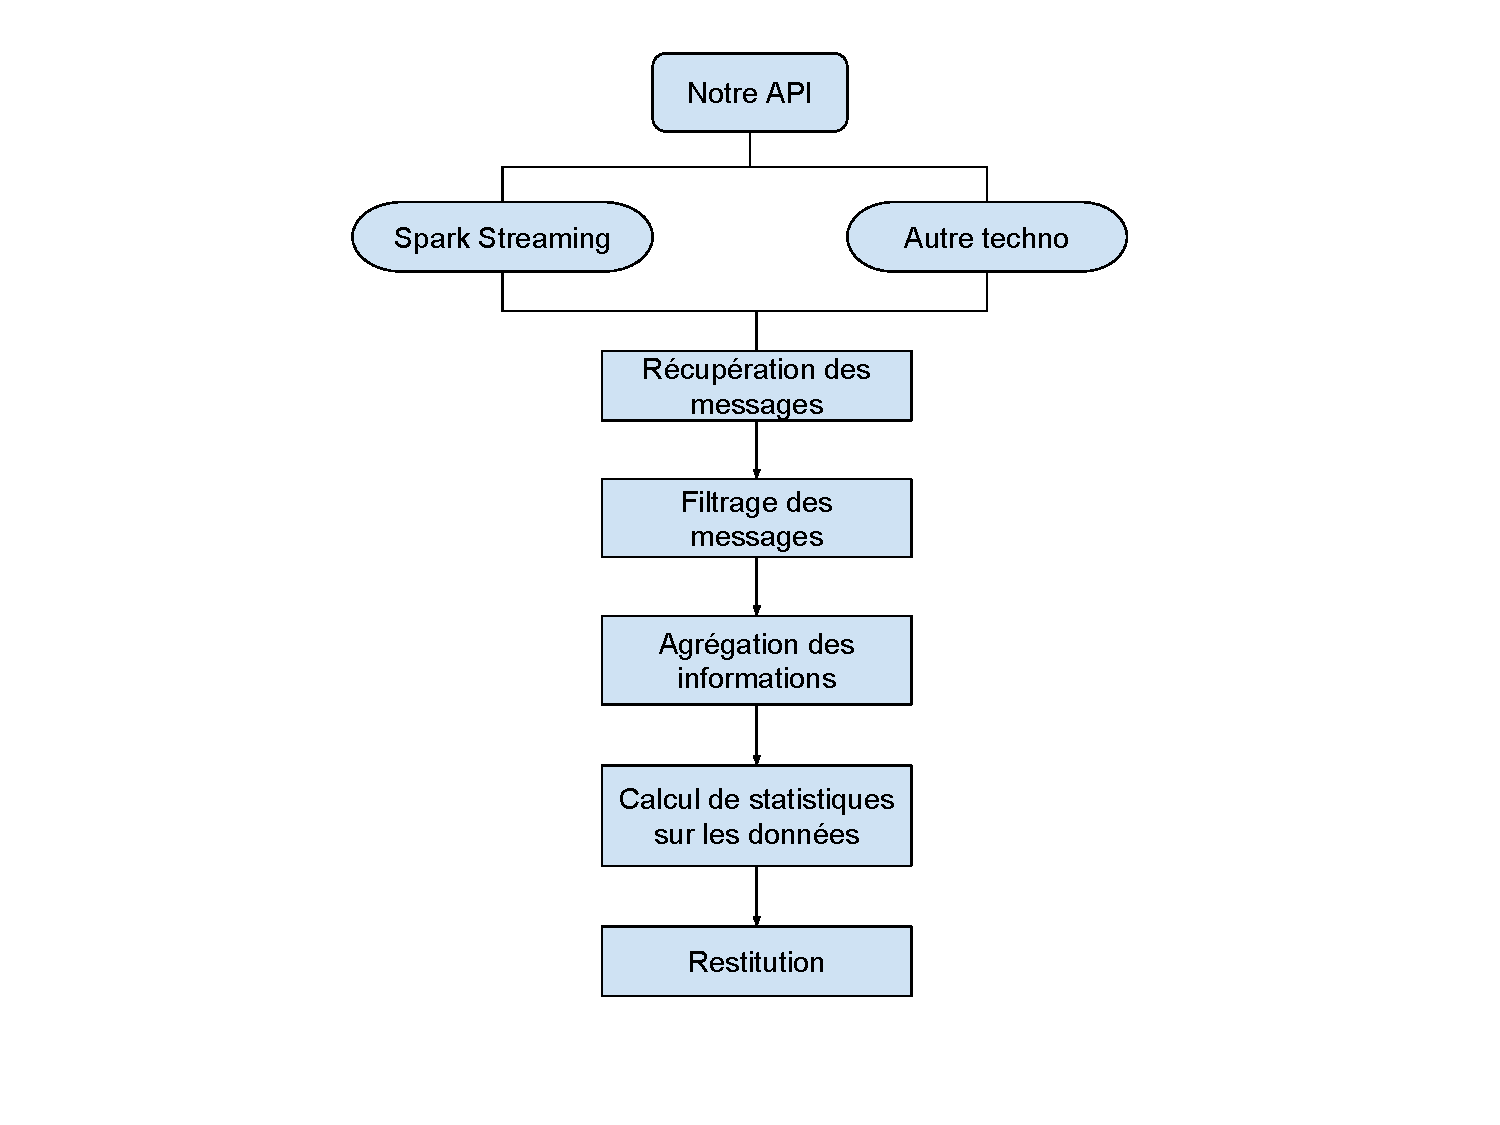
\includegraphics[width=1\textwidth]{images/WBS.pdf}
    \caption{WBF des prototypes}
    \label{WBS}
  \end{figure}


  \chapter{Partie C}
    \section{Résultats des métriques}
  L'intervalle entre chaque batch a été fixé à 1 seconde. Ainsi, Spark va récupérer pendant 1 seconde les tweets grâce à l'API de Twitter, effectuer les opérations de statistiques sur ces tweets et restituer l'information, dans notre cas, sous forme d'affichage à l'écran. Un diagramme de déploiement est présenté à la figure \ref{fig:digramme de déploiement}.

    \begin{figure}
        \centering
        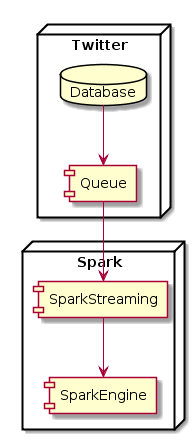
\includegraphics{images/diagramme-deploiement.png}
        \caption{Diagramme de déploiement}
        \label{fig:digramme de déploiement}
    \end{figure}

  \subsection{Time behaviour}
    Une des catégories de métriques est la notion de temps. En effet, pour l'analyse en temps réel, il est nécessaire de connaître les durées de chaque action afin de déterminer d'éventuel goulot d'étranglement. Pour notre prototype, nous avons mis en place une métrique sur la durée pour effectuer un batch complet, à savoir la récupération des tweets et le calcul de statistiques sur celui-ci. Une deuxième métrique a été mise en place dans le but de relever la durée nécessaire seulement pour réaliser les statistiques sur les tweets d'un batch. La figure~\ref{fig:resultats_stat_tweet} présente les résultats obtenus. \\

    \begin{figure}
      \centering
      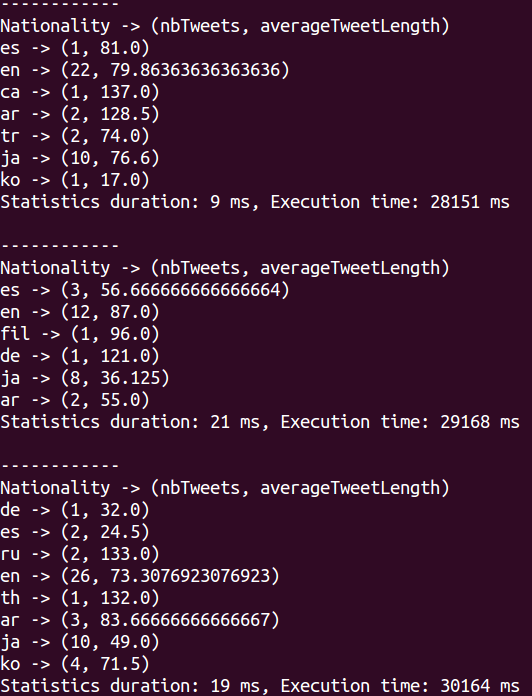
\includegraphics[width=0.6\textwidth]{images/stat_results.png}
      \caption{Résultats de l'analyse de tweet en temps réel}
      \label{fig:resultats_stat_tweet}
    \end{figure}

    Nous pouvons observer trois batch différents. Cela correspond donc à un temps d'exécution théorique de streaming de trois secondes (car nous avions spécifié un intervalle de 1 seconde comme paramètre). Cela est confirmer d'un point de vue exécution grâce à la métrique \emph{Execution time} présent sur la figure~\ref{fig:resultats_stat_tweet}. Nous pouvons remarquer que cette métrique prend respectivement les valeurs 28151, 29168 et 30164 millisecondes. Il y a donc bien 1 seconde entre chaque retour de résultats. \\

    \begin{figure}
      \centering
      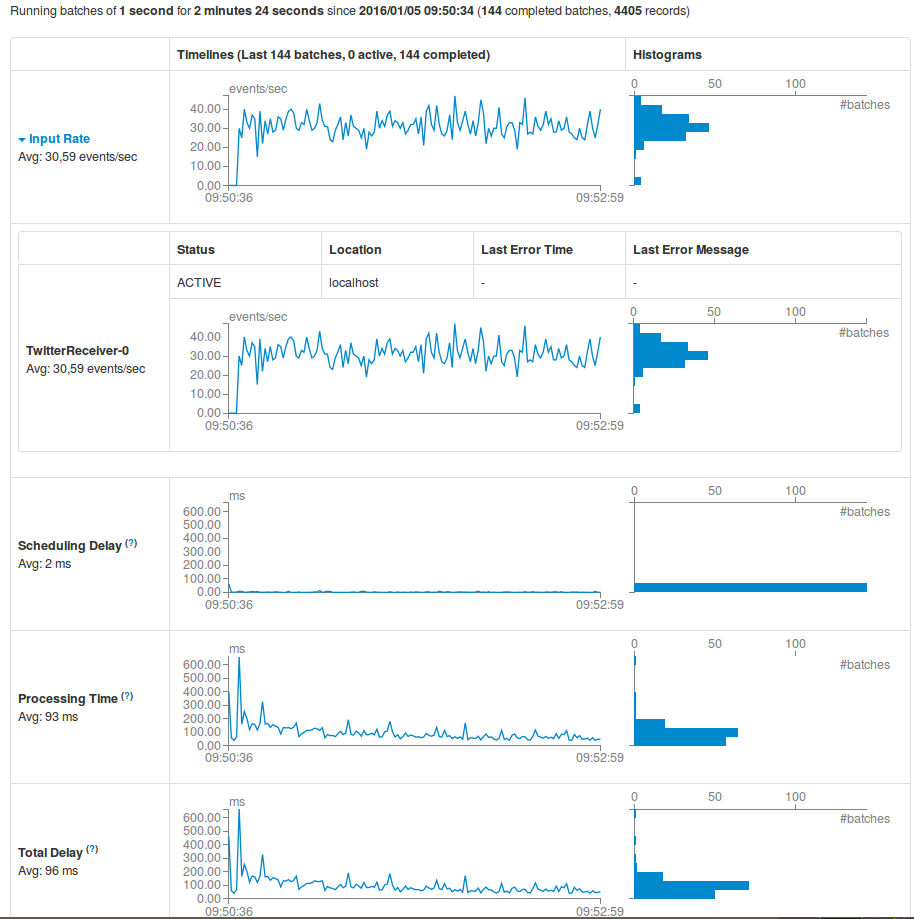
\includegraphics[width=1.0\textwidth]{images/streaming_spark_ui.png}
      \caption{Statistiques de Spark streaming}
      \label{fig:statistiques_spark_streaming_ui}
    \end{figure}

    Cependant, il serait intéressant de connaître la durée réelle de traitement d'un batch et non pas seulement la durée entre chaque batch qui est fixée manuellement. Spark possède une interface web regroupant de nombreuses métriques afin de suivre l'évolution de consommation de mémoire, le nombre de tâches effectuées, les erreurs… Ainsi la figure~\ref{fig:statistiques_spark_streaming_ui} présente ces résultats. La rubrique \emph{Processing Time} présente une moyenne de 104 ms pour traiter un batch dans son intégralité, ce qui est bien inférieur à la durée de 1s entre chaque batch et donc il n'y a pas de goulot d'étranglement. \\

    La deuxième métrique est nommée \emph{Statistics duration} est prend respectivement les valeurs 9, 21 et 19 millisecondes. Le temps de calcul des statistiques sur les tweets d'un batch est faible par rapport au temps de 104 ms nécessaire au traitement d'un batch. En effet, il y a peu de données à traiter et le temps restant est nécessaire au téléchargement des données depuis l'API de Twitter.

  \subsection{Resources utilization}
    \subsubsection{Vitesse de transmission}
      Une des métriques d'utilisation des ressources est la vitesse de transmission des messages entre l'API de Twitter et notre prototype. La figure~\ref{fig:statistiques_spark_streaming_ui} présente la catégorie \emph{Input Rate} qui correspond à la moyenne du nombre de Tweets par seconde. Cette valeur pour notre prototype est de 30,59 tweets par seconde.

    \subsubsection{Nombre d'erreurs}
      Une autre métrique était le nombre d'erreurs liés à la mémoire. La figure~\ref{fig:executor_spark_streaming_ui} présente des statistiques sur la mémoire des exécuteurs. Nous pouvons constater que la colonne \emph{Failed Tasks} a une valeur nulle et donc le prototype n'a pas eu d'erreur de mémoire.

      \begin{figure}
        \centering
        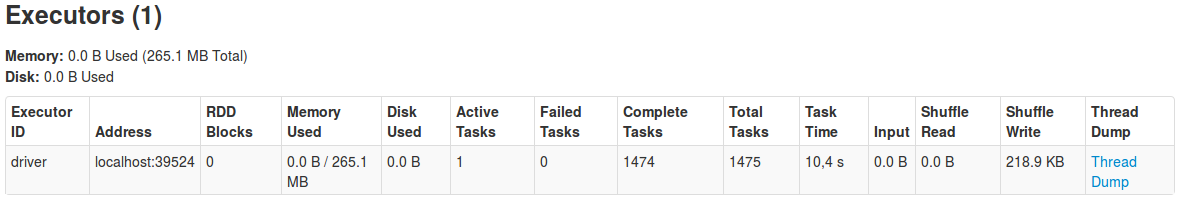
\includegraphics[width=1.0\textwidth]{images/executor_spark_ui.png}
        \caption{Statistiques liées à la mémoire}
        \label{fig:executor_spark_streaming_ui}
      \end{figure}

    \subsubsection{Pourcentage d'utilisation du CPU}
      Sur un ordinateur possédant un processeur Intel® Pentium(R) CPU P6100 @ 2.00GHz x 2, l'utilisation de notre prototype requiert 10\% du CPU.

  \subsection{Installability}
    \subsubsection{Installation du prototype}
      Afin d'utiliser le prototype, il est nécessaire d'installer 3 outils:
      \begin{itemize}
        \item Scala (\url{http://scala-lang.org/}), le langage utilisé pour l'implémentation du prototype
        \item Spark (\url{https://spark.apache.org/}), l'outil permettant le streaming avec l'API Twitter
        \item Sbt (\url{http://www.scala-sbt.org/}), un gestionnaire de dépendances
      \end{itemize}

    \subsubsection{Configuration du prototype}
      La seule étape de configuration du prototype est de récupérer les quatre tokens nécessaires à la connexion avec l'API de Twitter. La procédure est expliquée à cette adresse : \url{https://dev.twitter.com/oauth/overview/application-owner-access-tokens}.

    \subsubsection{Nombre de machine}
      L'utilisation de Spark streaming permet la gestion d'un nombre illimité de machines. Ainsi, plus le nombre de machines sera élevé et plus il sera possible de traiter un nombre de batch important, le tout avec un temps de traitement plus court. La procédure pour lancer le prototype sur un cluster de machine est disponible à cette adresse : \url{https://spark.apache.org/docs/latest/spark-standalone.html}.


	% Table des figures
	\listoffigures

	% Bibliographie
	% \bibliographystyle{abbrv}
	% \bibliography{src/bibli}

	% Annexes
	% \appendix
	% \section*{Annexes}
	% \input{}

	\pageQuatriemeCouverture{Département ASI}{+33 2 32 95 97 79}{asi@insa-rouen.fr}{}{}
\end{document}
